% ----------------------------------------------------------------- %
%             The Speech Signal Processing Toolkit (SPTK)           %
%             developed by SPTK Working Group                       %
%             http://sp-tk.sourceforge.net/                         %
% ----------------------------------------------------------------- %
%                                                                   %
%  Copyright (c) 1984-2007  Tokyo Institute of Technology           %
%                           Interdisciplinary Graduate School of    %
%                           Science and Engineering                 %
%                                                                   %
%                1996-2017  Nagoya Institute of Technology          %
%                           Department of Computer Science          %
%                                                                   %
% All rights reserved.                                              %
%                                                                   %
% Redistribution and use in source and binary forms, with or        %
% without modification, are permitted provided that the following   %
% conditions are met:                                               %
%                                                                   %
% - Redistributions of source code must retain the above copyright  %
%   notice, this list of conditions and the following disclaimer.   %
% - Redistributions in binary form must reproduce the above         %
%   copyright notice, this list of conditions and the following     %
%   disclaimer in the documentation and/or other materials provided %
%   with the distribution.                                          %
% - Neither the name of the SPTK working group nor the names of its %
%   contributors may be used to endorse or promote products derived %
%   from this software without specific prior written permission.   %
%                                                                   %
% THIS SOFTWARE IS PROVIDED BY THE COPYRIGHT HOLDERS AND            %
% CONTRIBUTORS "AS IS" AND ANY EXPRESS OR IMPLIED WARRANTIES,       %
% INCLUDING, BUT NOT LIMITED TO, THE IMPLIED WARRANTIES OF          %
% MERCHANTABILITY AND FITNESS FOR A PARTICULAR PURPOSE ARE          %
% DISCLAIMED. IN NO EVENT SHALL THE COPYRIGHT OWNER OR CONTRIBUTORS %
% BE LIABLE FOR ANY DIRECT, INDIRECT, INCIDENTAL, SPECIAL,          %
% EXEMPLARY, OR CONSEQUENTIAL DAMAGES (INCLUDING, BUT NOT LIMITED   %
% TO, PROCUREMENT OF SUBSTITUTE GOODS OR SERVICES; LOSS OF USE,     %
% DATA, OR PROFITS; OR BUSINESS INTERRUPTION) HOWEVER CAUSED AND ON %
% ANY THEORY OF LIABILITY, WHETHER IN CONTRACT, STRICT LIABILITY,   %
% OR TORT (INCLUDING NEGLIGENCE OR OTHERWISE) ARISING IN ANY WAY    %
% OUT OF THE USE OF THIS SOFTWARE, EVEN IF ADVISED OF THE           %
% POSSIBILITY OF SUCH DAMAGE.                                       %
% ----------------------------------------------------------------- %
\hypertarget{xgr}{}
\name{xgr}{XY-plotter simulator for X-window system}{plotting graphs}

\begin{synopsis}
 \item[xgr]   [ --s {\em S} ] [ --l ] [ --rv ] [ --m ] [ --bg {\em BG} ]
              [ --hl {\em HL} ] [ --bd {\em BD} ] 
 \item[\ ~~~~] [ --ms {\em MS} ] [ --g {\em G} ] [ --d {\em D} ]
              [ --t {\em T} ] [ {\em infile} ]
\end{synopsis} 

\begin{qsection}{DESCRIPTION}
{\em xgr} plots a graph from a sequence of FP5301 plotter commands, 
displaying the output on the screen in a new X window.

When the X window is created, 
the keyboard focus is initially assigned to that new window, 
which responds to a limited set of user interactions:
\begin{itemize}
\item Changing the window size truncates or expands the area 
	in which the graph is displayed, 
	but the graph remains the same size (i.e.
	it is not rescaled to fit the new window size).
\item If the graph is larger than the window, 
	the position within the window can be changed with 
	``vi'' cursor movement commands:
\begin{quote}
		h: left scroll\\
		j: down scroll\\
		k: up scroll\\
		l: right scroll
\end{quote}
\item To delete the window, type one of the following:
	``q'',``Ctrl-c'',``Ctrl-d''
\end{itemize}
\end{qsection}

\begin{options}
	\argm{s}{S}{shrink}{3.38667}
	\argm{l}{}{landscape}{FALSE}
	\argm{rv}{}{reverse mode}{FALSE}
	\argm{m}{}{monochrome display mode}{FALSE}
	\argm{bg}{BG}{background color}{white}
	\argm{hl}{HL}{highlight color}{blue}
	\argm{bd}{BD}{border color}{blue}
	\argm{ms}{MS}{mouse color}{red}
	\argm{g}{G}{geometry}{NULL}
	\argm{d}{D}{display}{NULL}
	\argm{t}{T}{window title}{xgr}
\end{options}
\begin{qsection}{EXAMPLE}
The following example uses \hyperlink{fdrw}{fdrw} to draw a graph based on data read
from {\em data.f}, and sends the output to a X-Window environment:
\begin{quote}
 \verb!fdrw < data.f | xgr!
\end{quote}
\begin{center}
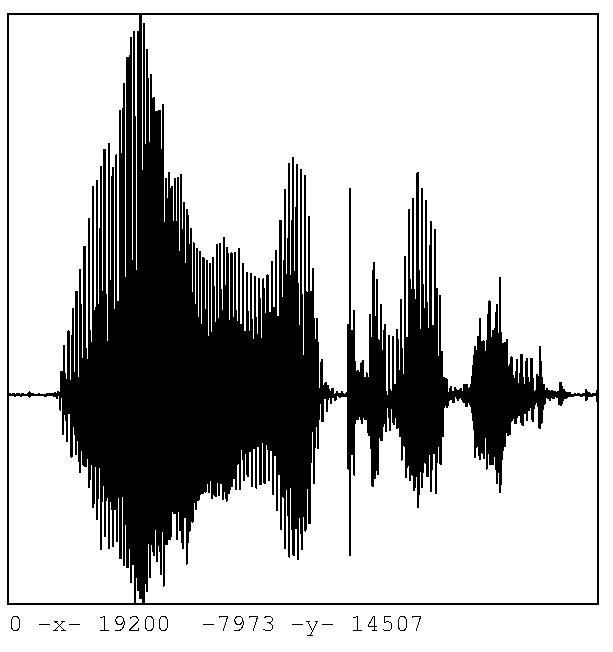
\includegraphics[width=6cm]{fig/xgr.pdf}
\end{center}
\end{qsection}
\begin{qsection}{NOTICE}
\begin{itemize}
\item If the display server does not contain backing store function,
then the hidden part of virtual screen is erased.

\item To reduce the waiting time to display graphs,
an image of virtual screen is copied to the memory.
If the size assigned by the --g option is too small
or if during the time the graph is being plotted another window
is put above the virtual screen, a part of the virtual screen
needs to be erased.
The --s option is suggested whenever the size of
the virtual screen should be reduced.
\end{itemize}

\end{qsection}
\begin{qsection}{SEE ALSO}
\hyperlink{fig}{fig},
\hyperlink{fdrw}{fdrw}
\end{qsection}
